
%%%%%%%%%%%%%%%%%%%%%%%%%%%%%%%%%%%%%%%%%%%%%%%%%%%%%%%%%%%%%%%%%%%%%%%%%%%%%%%%
\documentclass[letterpaper, 10pt, conference]{ieeeconf}

\IEEEoverridecommandlockouts
\overrideIEEEmargins

\usepackage{mathtools}
\usepackage{mathrsfs}
\usepackage{cite}
\usepackage{amsmath}
\usepackage{amssymb}
\usepackage{amsfonts}
\usepackage{graphicx}
\usepackage{adjustbox}
\usepackage{xcolor}
\usepackage[thmmarks, amsmath]{ntheorem}

\DeclareMathOperator{\diff}{d}
\newcommand{\ddt}{\tfrac{\diff}{\diff \! t}}
\providecommand{\norm}[1]{\lVert#1\rVert}

\newtheorem{theorem}{Theorem}
\newtheorem{lemma}{Lemma}
\newtheorem{proposition}{Proposition}
\newtheorem{assumption}{Assumption}
\newtheorem{remark}{Remark}
\newtheorem{definition}{Definition}
\newtheorem{corollary}{Corollary}

\title{\LARGE \bf
System Analysis and Torque Control of a 2-DOF Robot Arm
}

\author{Ashvin Anilkumar, Leo Xu}

\begin{document}

\maketitle
\thispagestyle{plain}
\pagestyle{plain}

%%%%%%%%%%%%%%%%%%%%%%%%%%%%%%%%%%%%%%%%%%%%%%%%%%%%%%%%%%%%%%%%%%%%%%%%%%%%%%%%

\begin{figure}[htbp]
    \centering
    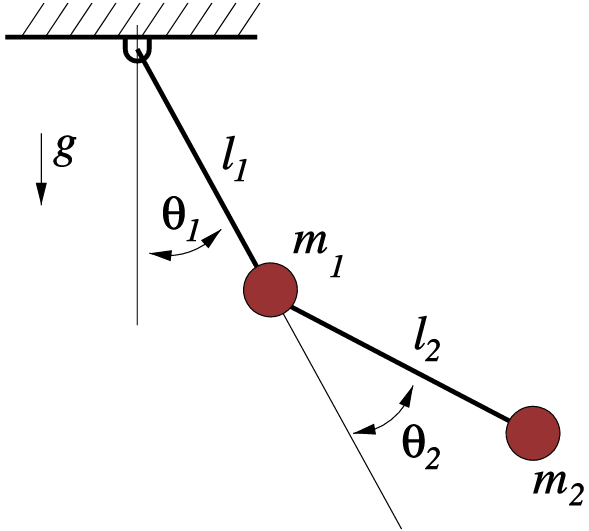
\includegraphics[width=0.25\textwidth]{simple_double_pend.png}
    \caption{Diagram of 2-DOF robot arm \cite{underactuated}.}
    \label{fig:arm}
\end{figure}

\section{Introduction \& Motivation}

In this project, we are interested in analyzing the
2-DOF robot arm shown in Figure \ref{fig:arm}.
The equations of motion for this system contain
nonlinear terms (sines and cosines) and serve as
a simple starting point for examining robot
manipulators. We will linearize the system about
an equilibrium point, examine its stability, and,
if time permits, design an admittance controller
for the robot.

\section{Mathematical Model \& Linearization}

As given by \cite{underactuated}, the equations
of motion (EOM) for a general robotic manipulator
with joint position vector $\mathbf{q}$,
where $\dim(\mathbf{q})=n$, are

\begin{equation}
\boxed{
\mathbf{M}(\mathbf{q})\ddot{\mathbf{q}}
+
\mathbf{C}(\mathbf{q},\dot{\mathbf{q}})
\dot{\mathbf{q}}
=
\boldsymbol{\tau}_g(\mathbf{q})
+
\mathbf{B}\mathbf{u}.
}
\label{eq:eom}
\end{equation}

Here,
$\mathbf{M}(\mathbf{q})\in\mathbb{R}^{n\times n}$
is the inertia matrix,
$\mathbf{C}(\mathbf{q},\dot{\mathbf{q}})
\in\mathbb{R}^{n\times n}$
captures Coriolis and centrifugal effects,
$\boldsymbol{\tau}_g(\mathbf{q})\in\mathbb{R}^{n}$
is the gravitational torque vector, and
$\mathbf{B}\in\mathbb{R}^{n\times m}$
maps the control inputs
$\mathbf{u}\in\mathbb{R}^{m}$
to generalized forces.

For the simple 2-DOF example
\cite{underactuated}, we have

\[
\adjustbox{max width=0.95\columnwidth}{$\displaystyle
\mathbf{M}(\mathbf{q}) =
\begin{bmatrix}
(m_1+m_2)l_1^2 + m_2l_2^2 + 2m_2l_1l_2c_2
&
m_2l_2^2 + m_2l_1l_2c_2
\\[6pt]
m_2l_2^2 + m_2l_1l_2c_2
&
m_2l_2^2
\end{bmatrix}
$}
\]

\[
\adjustbox{max width=0.95\columnwidth}{$\displaystyle
\mathbf{C}(\mathbf{q},\dot{\mathbf{q}}) =
\begin{bmatrix}
0
&
-m_2l_1l_2(2\dot{q}_1+\dot{q}_2)s_2
\\[6pt]
\frac{1}{2}m_2l_1l_2(2\dot{q}_1+\dot{q}_2)s_2
&
-\frac{1}{2}m_2l_1l_2\dot{q}_1s_2
\end{bmatrix}
$}
\]

\[
\adjustbox{max width=0.95\columnwidth}{$\displaystyle
\boldsymbol{\tau}_g(\mathbf{q}) =
-g
\begin{bmatrix}
(m_1+m_2)l_1s_1 + m_2l_2s_{1+2}
\\[6pt]
m_2l_2s_{1+2}
\end{bmatrix}
$}
\]

\[
\mathbf{B} =
\begin{bmatrix}
1 & 0\\
0 & 1
\end{bmatrix}
=\mathbf{I}_2.
\]

Here, we use the shorthand notation

\begin{align*}
c_2 &= \cos(q_2), &
s_1 &= \sin(q_1),\\
s_2 &= \sin(q_2), &
s_{1+2} &= \sin(q_1+q_2).
\end{align*}

For strictly positive masses and link lengths,
$\mathbf{M}(\mathbf{q})$ is positive definite
and therefore invertible.

We can isolate the joint accelerations as

\begin{equation}
\adjustbox{max width=0.80\columnwidth}{$\displaystyle
\ddot{\mathbf{q}} =
\mathbf{M}(\mathbf{q})^{-1}
\left[
-\mathbf{C}(\mathbf{q},\dot{\mathbf{q}})
\dot{\mathbf{q}}
+\mathbf{B}\mathbf{u}
+\boldsymbol{\tau}_g(\mathbf{q})
\right].
$}
\label{eq:acceleration}
\end{equation}

\subsection{Nonlinear State-Space Representation}

We define the state vector and control input as

\[
\mathbf{x} =
\begin{bmatrix}
q_1 & q_2 & \dot{q}_1 & \dot{q}_2
\end{bmatrix}^{T},
\qquad
\mathbf{u} =
\begin{bmatrix}
\tau_1 & \tau_2
\end{bmatrix}^{T}.
\]

Since $\mathbf{B}=\mathbf{I}_2$, we can
express the nonlinear state-space dynamics as

\begin{equation}
\boxed{
\dot{\mathbf{x}} =
\underbrace{
\mathbf{A}_0\mathbf{x}
+\mathbf{G}(\mathbf{x})\mathbf{u}
+\mathbf{h}(\mathbf{x})
}_{\mathbf{f}(\mathbf{x},\mathbf{u})}
}
\label{eq:nonlinear_ss}
\end{equation}

where

\[
\mathbf{A}_0 =
\begin{bmatrix}
0&0&1&0\\
0&0&0&1\\
0&0&0&0\\
0&0&0&0
\end{bmatrix},
\]

\[
\mathbf{G}(\mathbf{x}) =
\begin{bmatrix}
\mathbf{0}_{2\times2}\\
\mathbf{M}(x_2)^{-1}
\end{bmatrix},
\]

and

\[
\adjustbox{max width=0.95\columnwidth}{$\displaystyle
\mathbf{h}(\mathbf{x}) =
\begin{bmatrix}
\mathbf{0}_{2\times1}\\[4pt]
\mathbf{M}(x_2)^{-1}
\left[
\boldsymbol{\tau}_g(x_1,x_2)
-\mathbf{C}(\mathbf{x})
\begin{bmatrix}x_3\\x_4\end{bmatrix}
\right]
\end{bmatrix}.
$}
\]

Here, $\mathbf{M}(x_2)$,
$\mathbf{C}(\mathbf{x})$, and
$\boldsymbol{\tau}_g(x_1,x_2)$
refer to the previously defined manipulator
dynamics, expressed in terms of the state
variables.

The output consists of the two joint positions:

\begin{equation}
\boxed{
\mathbf{y} =
\mathbf{C}_y\mathbf{x}
+\mathbf{D}\mathbf{u}
}
\label{eq:output}
\end{equation}

where

\[
\mathbf{C}_y =
\begin{bmatrix}
1&0&0&0\\
0&1&0&0
\end{bmatrix},
\qquad
\mathbf{D}=\mathbf{0}_{2\times2}.
\]


\subsection{Linearization About Equilibrium}

We linearize the nonlinear system about the
downward-hanging equilibrium

\[
\mathbf{x}^* =
\begin{bmatrix}
0&0&0&0
\end{bmatrix}^{T},
\qquad
\mathbf{u}^* =
\begin{bmatrix}
0&0
\end{bmatrix}^{T}.
\]

At this equilibrium,

\[
\mathbf{f}(\mathbf{x}^*,\mathbf{u}^*)=
\mathbf{0}.
\]

Defining perturbations about the equilibrium,

\[
\delta\mathbf{x}
=\mathbf{x}-\mathbf{x}^*,
\qquad
\delta\mathbf{u}
=\mathbf{u}-\mathbf{u}^*,
\]

the first-order Taylor approximation gives

\begin{equation}
\boxed{
\delta\dot{\mathbf{x}}
=
\mathbf{A}\delta\mathbf{x}
+
\mathbf{B}_{\mathrm{lin}}\delta\mathbf{u}.
}
\label{eq:linear_ss}
\end{equation}

The linearized system matrices are obtained
from the Jacobians

\begin{align}
\mathbf{A}
&=
\left.
\frac{\partial\mathbf{f}}{\partial\mathbf{x}}
\right|_{\mathbf{x}^*,\mathbf{u}^*},
\label{eq:jacobian_A}
\\
\mathbf{B}_{\mathrm{lin}}
&=
\left.
\frac{\partial\mathbf{f}}{\partial\mathbf{u}}
\right|_{\mathbf{x}^*,\mathbf{u}^*}.
\label{eq:jacobian_B}
\end{align}

Evaluating these Jacobians at the equilibrium,
the linearized system matrix is

\[
\adjustbox{max width=0.95\columnwidth}{$\displaystyle
\mathbf{A} =
\begin{bmatrix}
0&0&1&0\\[4pt]
0&0&0&1\\[4pt]
-\dfrac{g}{l_1}
&
\dfrac{gm_2}{m_1l_1}
&0&0\\[10pt]
\dfrac{g}{l_1}
&
-\dfrac{g[m_1l_1+m_2(l_1+l_2)]}
{m_1l_1l_2}
&0&0
\end{bmatrix}
$}
\]

and the linearized input matrix is

\[
\adjustbox{max width=0.95\columnwidth}{$\displaystyle
\mathbf{B}_{\mathrm{lin}} =
\frac{1}{m_1m_2l_1^2l_2^2}
\begin{bmatrix}
0&0\\
0&0\\
m_2l_2^2&-m_2l_2(l_1+l_2)\\
-m_2l_2(l_1+l_2)&
m_1l_1^2+m_2(l_1+l_2)^2
\end{bmatrix}
$}
\]

The linearized output equation is

\begin{equation}
\boxed{
\delta\mathbf{y}
=
\mathbf{C}_y\delta\mathbf{x}
+
\mathbf{D}\delta\mathbf{u}.
}
\label{eq:linear_output}
\end{equation}

The output matrices remain

\[
\mathbf{C}_y =
\begin{bmatrix}
1&0&0&0\\
0&1&0&0
\end{bmatrix},
\qquad
\mathbf{D}=\mathbf{0}_{2\times2}.
\]

The resulting fourth-order linear
time-invariant (LTI) system describes the
local dynamics of the robot arm near the
downward equilibrium.

We will analyze its eigenvalues to characterize
local stability and examine the controllability
and observability of the linearized system.


\bibliographystyle{IEEEtran}
\bibliography{mybibfile}

\end{document}
